\documentclass[11pt,twocolumn]{article}

\usepackage{url}
\usepackage{graphicx}
\usepackage{indentfirst}
\usepackage{titlesec}
\usepackage{geometry}
% \usepackage[showframe]{geometry}
\usepackage{layout}

\geometry{top=80pt, bottom=80pt}

\titlespacing*{\section}{0pt}{14pt}{6pt}
\titlespacing*{\subsection}{0pt}{7pt}{6pt}

\setlength{\headsep}{0pt}

\titleformat{\section}
  {\normalfont\scshape}{\thesection}{1em}{}

\titleformat{\subsection}
  {\normalfont\scshape}{\thesubsection}{1em}{}

\newenvironment{boldenv}
  {\bfseries}

\begin{document}

\title{Robust Lens Flare Removal}
\author{Floris Chabert}
\date{}
\maketitle

\begin{abstract}\begin{boldenv}

\end{boldenv}\end{abstract}

\section{Motivation}

Lens flare and ghosting can be prevalent artifacts when taking pictures of a scene with a direct bright light. Those artifacts are usually caused by internal reflections of the lens due to a thin anti reflective coating and can easily ruin a beautiful picture.
\\

This project aims at automatically removing those lens artifacts via post-processing from a single input image to produce a restored picture. We designed an algorithm involving two steps: flare detection and recovery of the damaged region.

\section{Related Work}

Previous work found in the image processing literature around flare detection and more general flares detection can be separated in two categories: semi-automatic or using multiple images. Flare detection algorithms involve either having a manual step where the user has to select the general area where the flare is present[1] or the specific color of the flare. This prevents false positive and makes the algorithm more robust.
The second kind uses multiple pictures to detect flares. Some use images with different exposures to be able to find the spots that saturated the sensor. Others use multiple frames with camera motion in between to figure out where the artifact is [2]. One other interesting category uses pictures with and without flash to detect general flares.
\\

Various methods for recovery exist[3]. They are often referenced to as inpainting algorithms. Two major kind of inpainting are extensively documented: non-texture inpainting - often using partial differential equations based on different diffusion models[6][7] - and texture based methods[4]. Non texture based techniques usually work very well for small regions - especially when using higher degree gerivatives to preserve edges - but have a tendency to produce blurred patches. Texture based inpainiting works better to fill larger holes as they copy-paste patches to recover the image by minimizing some error metric.

\section{Method}

Here we aim at an automatic detection of the flares using a single input image. This involve a custom blob detection algorithm based on a concept used in OpenCV[5] tuned for the specific lens flares we want to recover and a hybrid inpainting method called exemplare-based inpainting[8].

\subsection{Detection}

The chosen detection algorithm used involve five main steps:
\\

\begin{figure}[ht!]
\centering
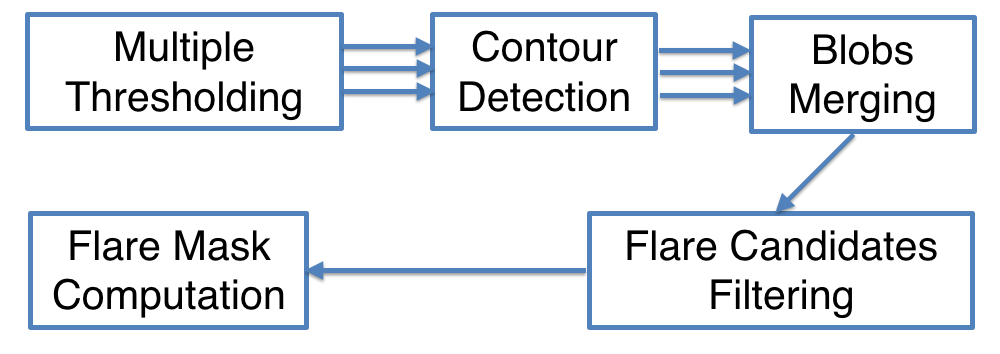
\includegraphics[width=72mm]{flow_detection.png}
\caption{Flare detection algorithm}
\end{figure}

\textbf{Multiple Thresholding} The image is converted to grayscale and binarized using a range of thresholds.
\\

\textbf{Contour Detection} For each binary image, we then find the contours using a border following method[9].
\\

\textbf{Blob Merging} The center of each blob is then computed and blobs from the different binary images are merged depending on their distance and radius. We finally obtain a set of potential flare candidates.
\\

\textbf{Flare Candidates Filtering} The flare candidates are pruned using various metrics which parameters have been tuned using a set of images as to be robust while avoiding false positive. Those metrics include cicrularity of the blob, convexity, inertia and area.

\begin{figure}[ht!]
\centering
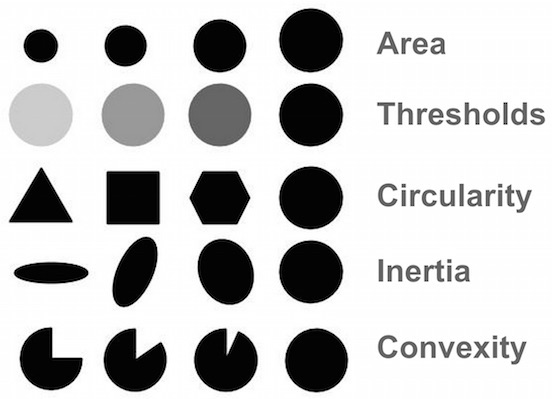
\includegraphics[width=72mm]{Filters.jpg}
\caption{Impact of filtering parameters for blob detection[5]}
\end{figure} 

\textbf{Flare Mask Computation} Finally the mask selecting the flares is computed for the next step.

\subsection{Recovery}

After the flare mask has been computed we can recover the damaged area using exemplar-based inpainting.

\begin{figure}[ht!]
\centering
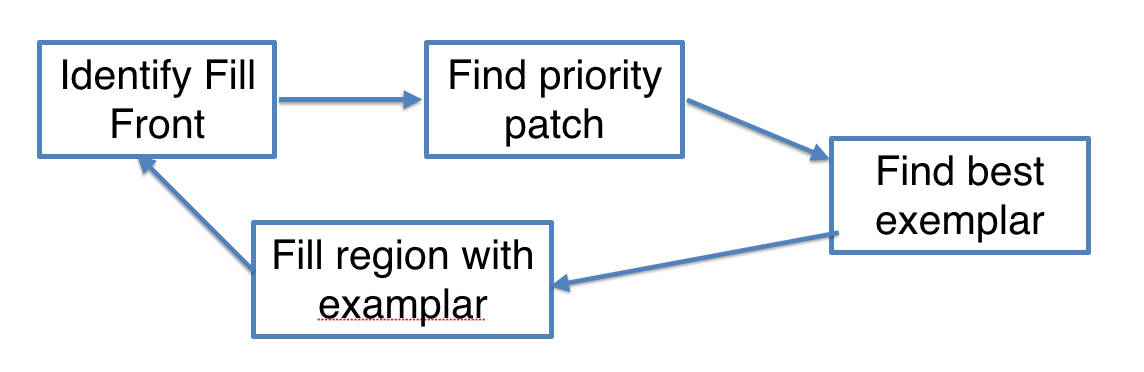
\includegraphics[width=72mm]{flow_inpainting.png}
\caption{Flare inpainting algorithm}
\end{figure}

After selecting a window around the flare - to avoid searching over the whole image, assuming good texture candidates are near the missing pixels - we execute the following algorithm until all the pixels have been recovered:
\\

\textbf{Identify Fill Front} We first find the contour of the region we want to fillb.
\\

\textbf{Identify Priority Patches} Patches on the fill front are assigned priorities as to priviledge patches that continue strong edges and are surrounded by high confidence pixels.
\\

\textbf{Find Best Exemplar} By priority order, we then search the window for known patches that minimize the error.
\\

\textbf{Fill Region using Exemplar Patch} We finally select pixels from the best patch to fill the masked pixels in the current patch to recover.

\begin{figure}[ht!]
\centering
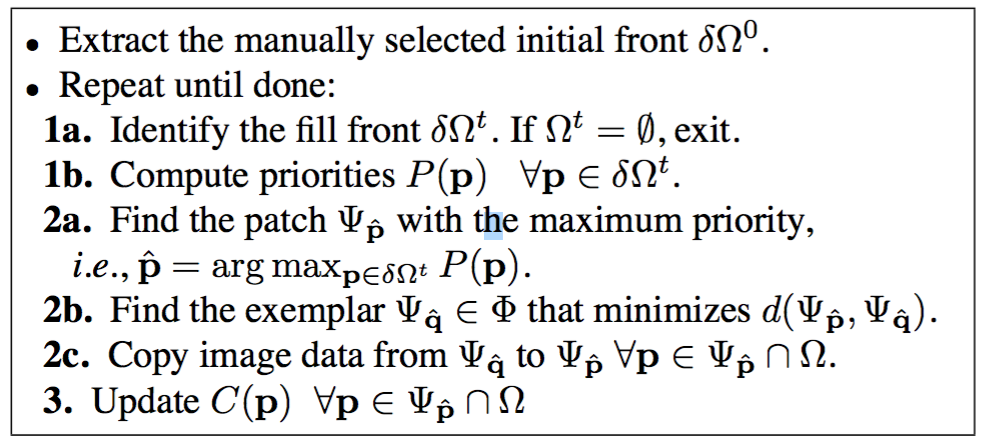
\includegraphics[width=72mm]{algo_inpainting.png}
\caption{Exemplar-based inpainting steps[8]}
\end{figure}

\section{Results}


\begin{figure}[ht!]
\centering
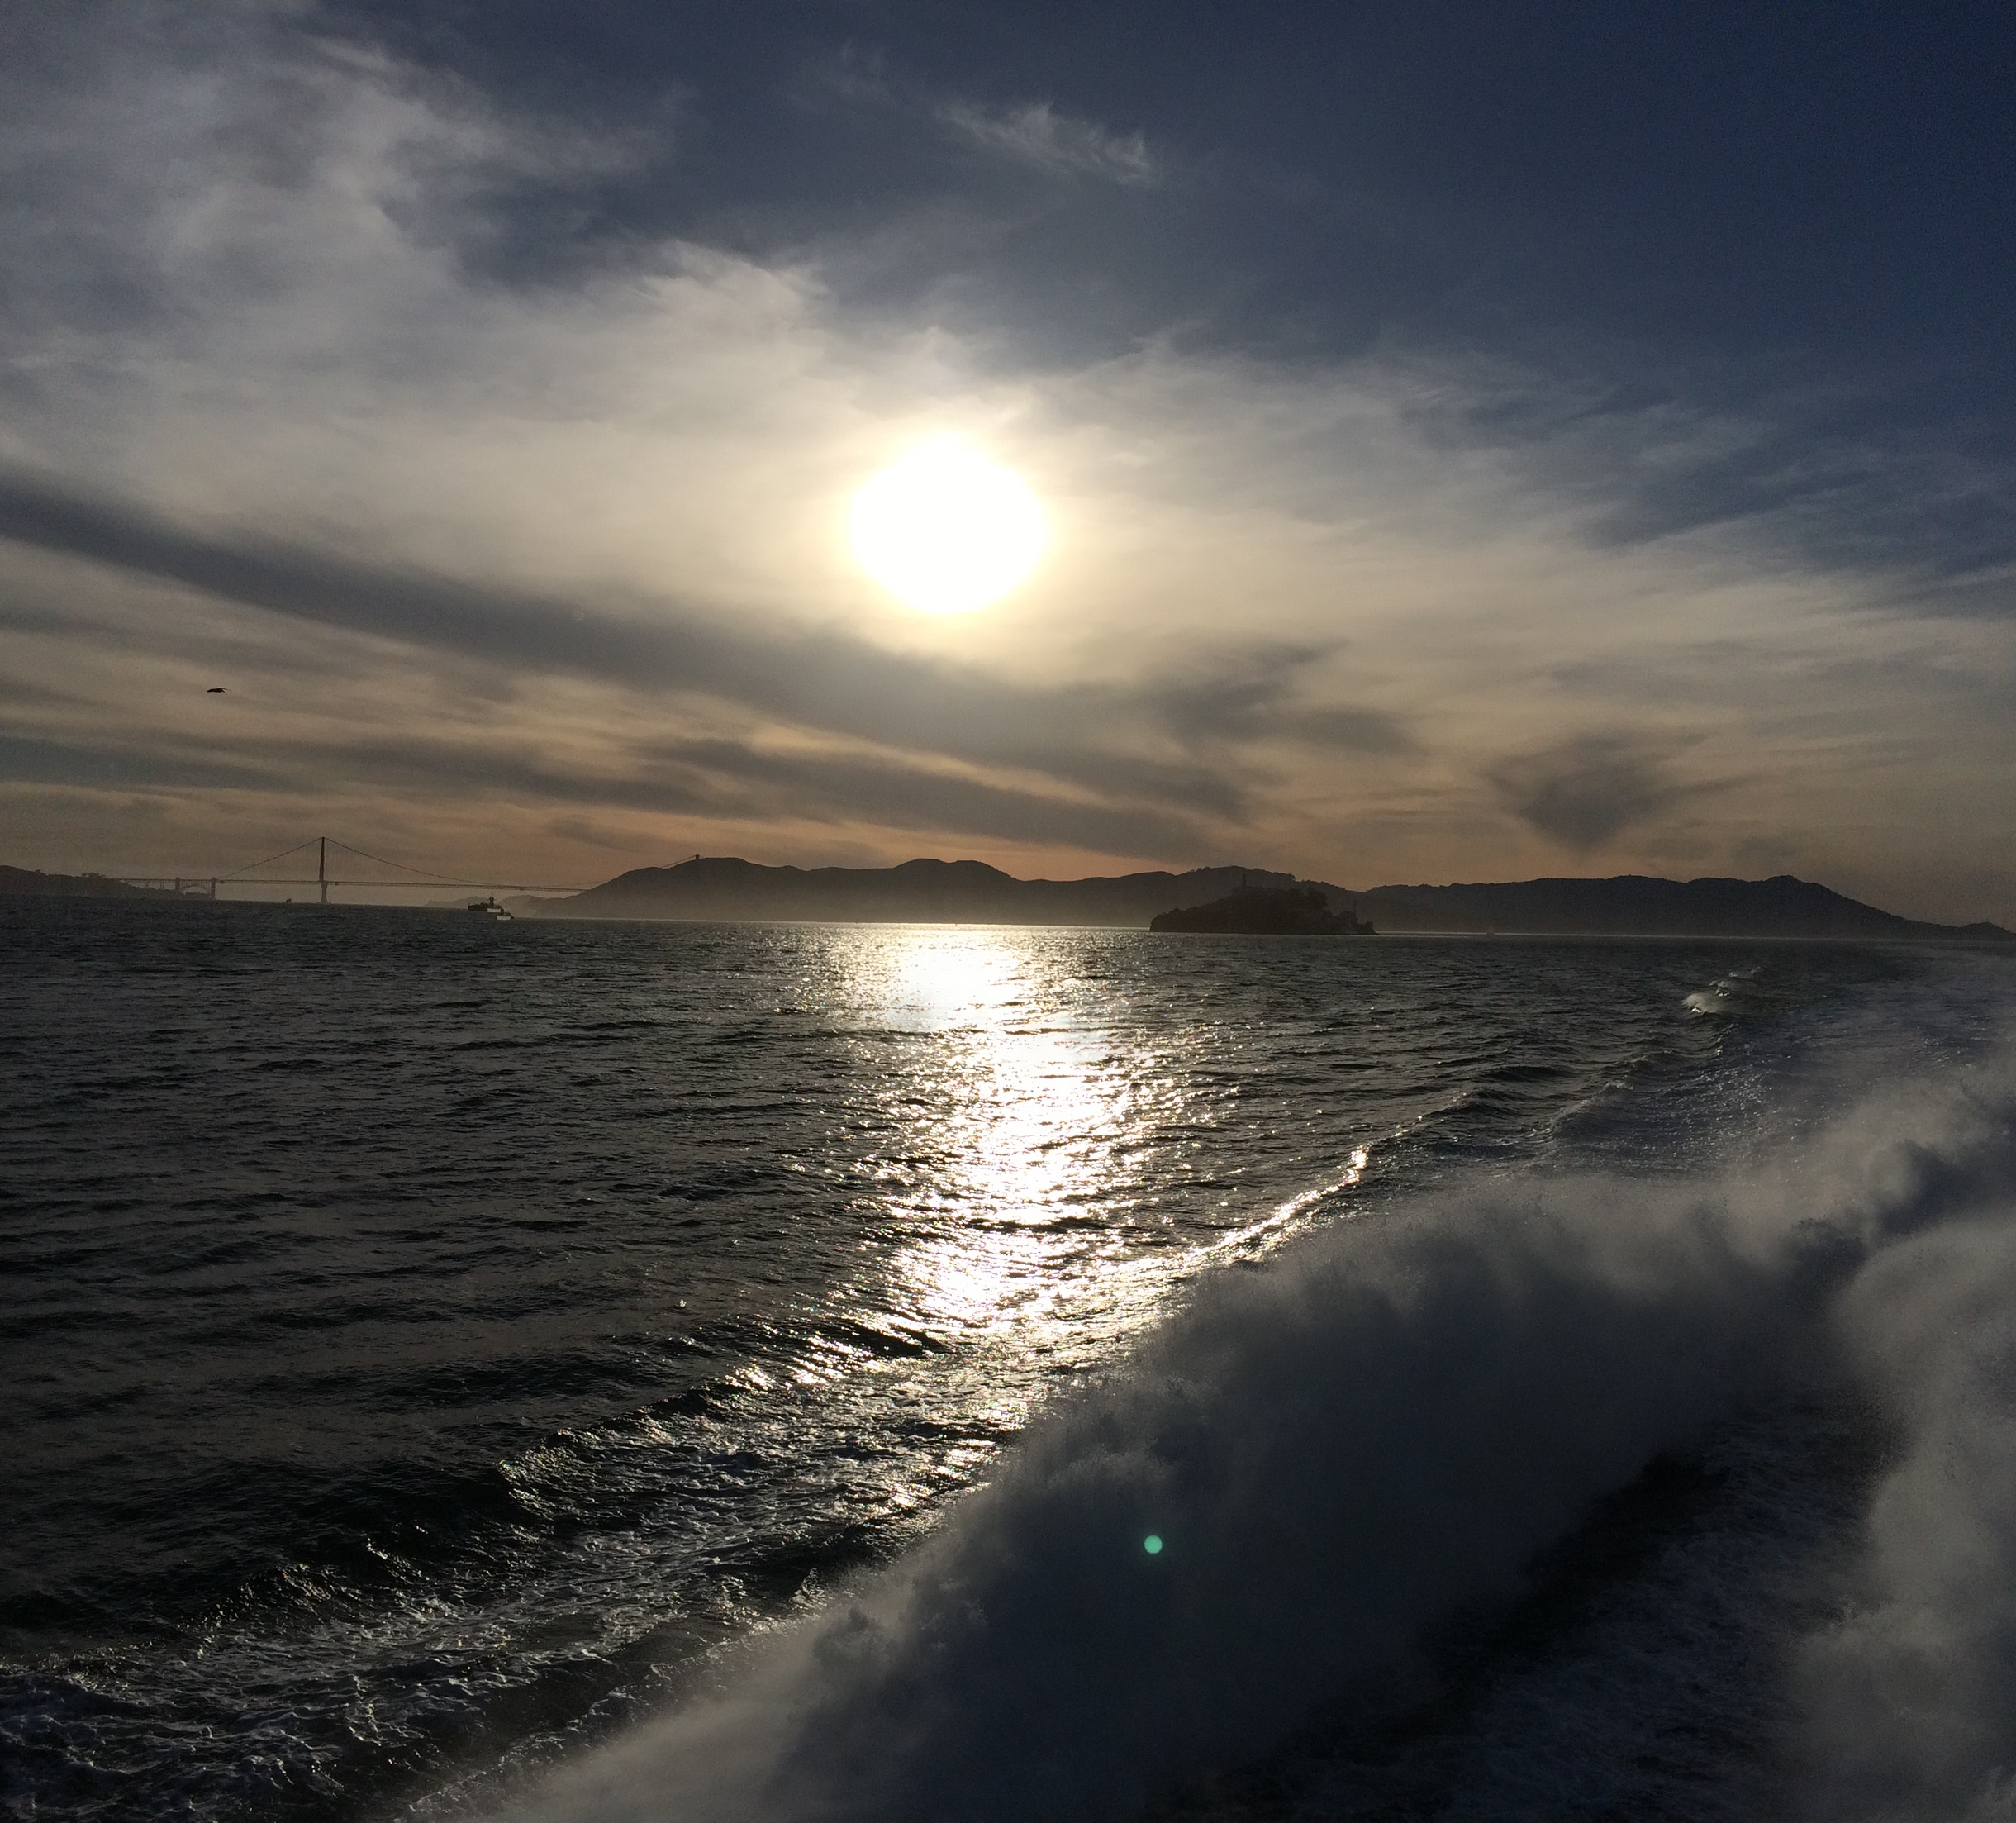
\includegraphics[width=72mm]{../Matlab/Images/1.jpg}
\caption{Pictures with lens flare artifact}
\end{figure}

\section{Discussion}


\begin{thebibliography}{1}

\bibitem
Dusan Psotny,
\emph{Removing lens flare from digital photographs},
Charles University in Prague, Diploma Thesis

\bibitem
Andreas Nussberger, Helmut Grabner, Luc Van Gool,
\emph{Robust Aerial Object Tracking in Images with Lens Flare},
Comput. Vision Lab., ETH Zurich

\bibitem
Marcelo Bertalmo, Vicent Caselles, Simon Masnou, Guillermo Sapiro,
\emph{Inpainting}

\bibitem
Rajul Suthar, Mr. Krunal R. Patel,
\emph{A Survey on Various Image Inpainting Techniques to Restore Image},
Int. Journal of Engineering Research and Applications

\bibitem
Aatya Mallick
\emph{Blob Detection Using OpenCV},
learnopencv.com

\bibitem
Tony F. Chan, Jianhong Shen
\emph{Mathematical Models for Local Nontexture Inpaintings}
SIAM Journal on Applied Mathematics, Vol. 62, No. 3

\bibitem
Tony F. Chan, Jianhong Shen,
\emph{Non-Texture Inpainting by Curvature-Driven-Diffusions},
Visual Comm Image Rep 06/2001

\bibitem
Jiansheng Liu, Mingming Li, Fangfang He
\emph{Region Filling and Object Removal by Exemplar-Based Image Inpainting},
IEEE Transactions on Image Processing, Vol. 13, No. 9, 2004

\bibitem
Suzuki, S. and Abe, K., 
\emph{Topological Structural Analysis of Digitized Binary Images by Border Following}
CVGIP 30 1, pp 32-46, 1985

\end{thebibliography}

\end{document}